\documentclass[a4paper,12pt]{article}

\usepackage{authblk}
\usepackage{geometry}
\usepackage{graphicx}
\usepackage{times}
\usepackage{titlesec}
\usepackage{tocloft}
\usepackage{float}
\usepackage[colorlinks=true, allcolors=black]{hyperref}
\usepackage[backend=biber, style=authoryear, sorting=none]{biblatex}
\addbibresource{refs.bib}

\geometry{left = 1.5in, right = 1.25in, top = 1.25in, bottom = 1.25in, headheight=0.5in, footskip=0.5in}
\renewcommand{\baselinestretch}{1.5}
\setlength{\parskip}{18pt}
\setlength{\parindent}{0pt}

\titleformat{\section}{\bfseries\fontsize{16pt}{18pt}\selectfont}{Chapter \thesection}{1em}{}
\titlespacing{\section}{0pt}{0pt}{-10pt}
\titleformat{\subsection}{\bfseries\fontsize{14pt}{16pt}\selectfont}{\thesubsection}{1em}{}
\titlespacing{\subsection}{0pt}{-10pt}{-20pt}
\titleformat{\subsubsection}{\bfseries\fontsize{13pt}{15pt}\selectfont}{\thesubsubsection}{1em}{}
\titlespacing{\subsubsection}{0pt}{-10pt}{-20pt}
\titleformat{\paragraph}{\bfseries\fontsize{12pt}{14pt}\selectfont}{\theparagraph}{1em}{}

\renewcommand{\cftsecpresnum}{Chapter }
\renewcommand{\cftsecaftersnum}{}
\renewcommand{\cftsecaftersnumb}{\quad}
\setlength{\cftsecnumwidth}{4em}

\setcounter{secnumdepth}{4}
\setcounter{tocdepth}{4}
\renewcommand{\contentsname}{Table of Contents}
\renewcommand{\cftsecleader}{\cftdotfill{\cftdotsep}}
\renewcommand{\cftdotsep}{1}

\AtEveryBibitem{
    \clearfield{url}
    \clearfield{doi}
}

\title{
\textbf{
    Kathmandu University \\
    \large{Department of Artificial Intelligence}\\
    \normalsize{Panchkhal, Kavre}\\[1.5cm]}
    
\includegraphics[width=3cm]{KU-Logo.png}\\[1cm]
    \normalsize{A Project Proposal\\on\\
    \textbf{"Research Space"}}\\[0.5cm]
    \normalsize{[Code No.: AISP 301]\\
    (For partial fulfillment of III/I Year/Semester in Artificial Intelligence)}\\[1cm]
}

\author[ ]{\normalsize{
        Submitted by: \linebreak
        Sujal Bajracharya(Roll no. 4)\linebreak
        Ashim Shrestha(Roll no. 22)\linebreak
        Yajjyu Tuladhar(Roll no. 27)
}}

\affil[ ]{\vspace{0.3cm}}
\affil[ ]{\normalsize{
        Submitted to: \linebreak
        Subodh Acharya \linebreak
        Department of Artificial Intelligence
}}

\date{\normalsize{Submission Date: \today}}

\begin{document}

\newgeometry{margin = 0.5 in}
\maketitle
\thispagestyle{empty}
\restoregeometry

\newpage
\setcounter{page}{1}
\pagenumbering{roman}

\section*{Abstract}
\addcontentsline{toc}{section}{\textit{Abstract}}
\newpage

\addcontentsline{toc}{section}{\textit{Table of Contents}}
\tableofcontents
\newpage

\addcontentsline{toc}{section}{\textit{List of Figures}}
\listoffigures
\newpage

\section*{Acronyms/Abbreviations}
\addcontentsline{toc}{section}{\textit{Acronyms/Abbreviations}}
\newpage

\setcounter{page}{1}
\pagenumbering{arabic}

\section{Introduction}
\subsection{Background}
In today's digital age, the abundance of academic literature can be overwhelming
for researchers and upcoming students seeking relevant information. Finding relevant
papers in specific domains is increasingly challenging due to the volume of
publications and the lack of efficient tools for personalized recommendations. Also
in fields like AI the velocity of new publications is so high that if you are not
reading everyday you fall behind. To address this challenge, an academic research
recommendation can streamline the process by utilizing citation networks and
semantic search for promising discovery processes, while the LLMs can provide
unprecedented capabilities in information retrieval and summarization.

\subsection{Problem Statement}
Current academic research platforms struggle to provide relevant paper
recommendations due to limitations in traditional keyword-based search methods.
These methods often fail to account for the detailed relationships between papers,
leading to information overload and inefficiency in literature discovery. Also many
papers don't explain the information that they learned from the documents they
have cited. This makes research tedious as to understand one academic paper you
will have to read multiple other papers too.

\subsection{Objectives}
The project aims to transform how researchers navigate and engage with academic
literature by developing an LLM-powered system that integrates citation networks,
knowledge graphs, and user-centric design. Our project aim to fulfill the following tasks:
\vspace{-25pt}
\begin{itemize}
    \item To retrieve papers relevant to user queries using a hybrid approach.
    \vspace{-10pt}
    \item Rank recommendations based on citation impact and semantic similarity.
    \vspace{-10pt}
    \item Explain papers using GraphRag.
\end{itemize}

\subsection{Motivation and Significance}
We ourselves have been reading or trying to read academic papers to understand AI
and its current advancements but we have found that current academic research platforms
like google scholar, arxiv, etc are not so easy to use if we want to read the cited
papers as well. For that we found connected papers to be slightly better as it
visualises the paper as a graph with its cited papers but understanding the paper
completely is still a challenge and using LLMs like chatgpt, deepseek only gives
partially correct or sometimes completely wrong answers.
\newpage

\section{Related Works}
Recommender Systems (RS) are one of the most popular and important applications of
Artificial Intelligence (AI). They have been widely adopted to help the users of
many popular content sharing and e-Commerce web sites to more easily find relevant
content, products or services. Meanwhile, Graph Learning (GL), which relates to
machine learning applied to graph structure data, is an emerging technique of AI
which is rapidly developing and has shown its great capability in recent years
\parencite{wang2021graphlearningbasedrecommender}.

Many researchers have explored graph-based recommendation methods. For instance,
\parencite{10.1145/3292500.3330673} employed a path-based approach for intent
recommendation to automatically recommend user intent according to user
historical behaviors without any input when users open the App,  similarly
\parencite{song2022ekarexplainablemethodknowledge} also proposed a path based
reinforcement learning method by formulating recommendation as a sequential
decision process. While \parencite{10.1145/3109859.3109889} utilized an embedding-based
method. Similarly, \parencite{10.1145/2939672.2939673} also used an embedding-based
technique by exploiting the knowledge base, to design three components to extract items'
semantic representations from structural content, textual content and visual content,
respectively.

\parencite{10.1145/2939672.2939673} used the TransR which was proposed by
\parencite{10.3233/JIFS-202177} which is a modification to the original TransE proposed
by \parencite{NIPS2013_1cecc7a7}.  TransE and TransR are both methods to represent
knowledge graphs (like "Paris is capitalof France") as numerical vectors for AI.
TransE treats relationships as simple translations in one shared space
(e.g., "Paris + capitalof = France"). It’s fast but struggles with complex
relationships (e.g., one person writing many books). TransR fixes this by first
projecting entities (like "Paris") into a custom space for each relationship before
translating, making it better for tricky cases but slower. Think of TransE as a
one-size-fits-all map, while TransR uses different maps for different roads.

Graph based methods have also been researched for academic paper recommendation.
\parencite{liu2025academicliteraturerecommendationlargescale} proposed a hybrid
recommendation framework for scientific article recommendation by constructing a
large-scale citation network comprising 190,381 articles from 70 journals spanning
statistics, econometrics, and computer science from 1981 to 2022. The framework
integrates network-based citation patterns with content-based semantic similarities.
To enhance content-based recommendations, OpenAI’s text-embedding-3-small model was
employed to generate embedding vectors for article abstracts, ensuring computational
efficiency and embedding stability for handling dynamic academic databases.

Another study, \parencite{church2024academicarticlerecommendationusing} explored the
complementary nature of content-based filtering (CBF) and graph-based methods (GB)
in academic search recommendations. They described how CBF analyzes abstracts to
infer authors’ positions, while GB examines citations to capture audience responses.
Their study identified nine key differences between CBF and GB, highlighting
synergistic opportunities for hybrid approaches. Notably, they utilized two
embedding techniques: Specter
\parencite{cohan-etal-2020-specter}, a BERT-based model
for encoding abstracts, and ProNE \parencite{zhang2019prone}, a spectral clustering-based method applied to
over 200M papers and 2B citations from Semantic Scholar.
As research in recommender systems advances, Retrieval-Augmented Generation (RAG)
presents a promising approach to enhancing the explainability and interpretability
of academic papers and recommendation methods. RAG combines retrieval mechanisms
with generative models to dynamically generate responses based on external knowledge
sources, making it an effective tool for summarizing and interpreting complex
research articles. RAG fails on global questions directed at an entire text corpus,
such as “What are the main themes in the dataset?”, since this is inherently a
query-focused summarization (QFS) task, rather than an explicit retrieval task
\parencite{edge2025localglobalgraphrag}.

\parencite{edge2025localglobalgraphrag} proposed GraphRAG, a graph-based approach
to question answering over private text corpora that scales with both the generality
of user questions and the quantity of source text.
\newpage

\section{Design and Implementation}
\subsection{Data Collection}
Datasets will be collected from reliable sources like arXiv using their public API,
Semantic Scholar’s S2ORC. After the dataset has been collected most of it will
already be in structured format except the PDFs of the papers. For the pdfs we will
parse and extract relevant textual information from it.

\subsection{Graph Construction and Storage}
\subsubsection{Citation Graph}
The citation graph represents papers as nodes and citation links as directed edges,
where an edge from Paper A to Paper B indicates that A cites B. This graph will be
implemented using NetworkX for rapid prototyping and small-scale analysis or Neo4j
for handling larger datasets with efficient querying capabilities.
\begin{figure}[H]
    \centering
    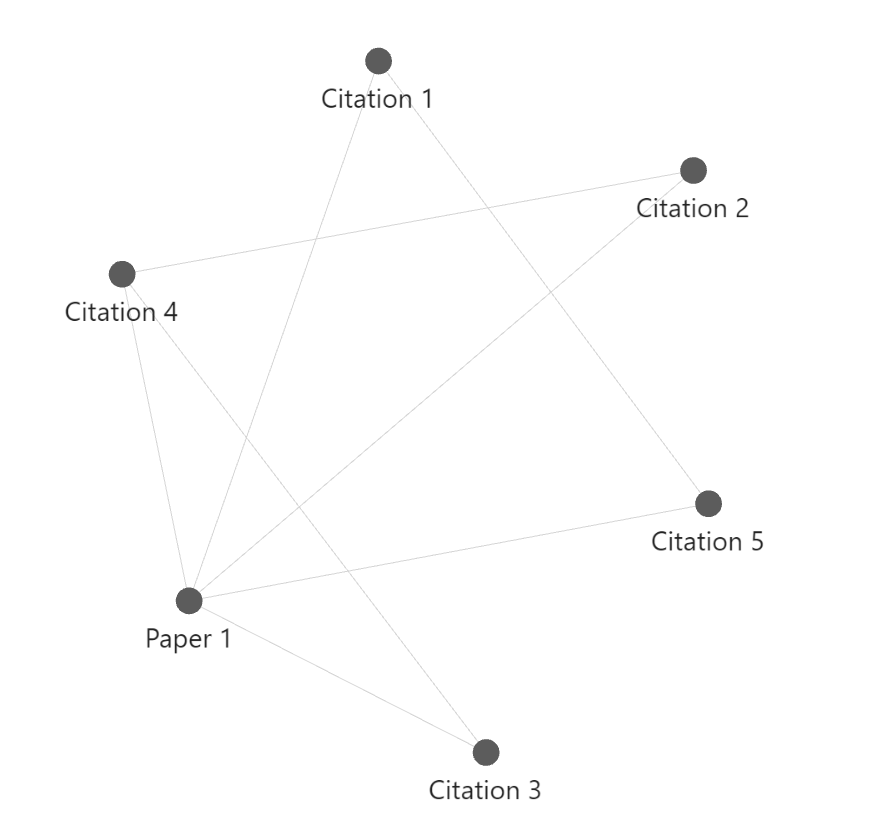
\includegraphics[width=10cm]{citationgraph.png}
    \caption{Example citation graph with dummy nodes}
\end{figure}

\subsubsection{Knowledge Graph}
Knowledge Graph will extend the citation graph by incorporating additional
information: author networks (edges between co-authors), subject networks(edges
to papers of the same subject), and topic embeddings (vector representations of
paper content derived from paper). This multi-layered graph provides a holistic
view of academic connections, enabling more nuanced retrieval by linking papers
through authors, and topics beyond direct citations.
\begin{figure}[H]
    \centering
    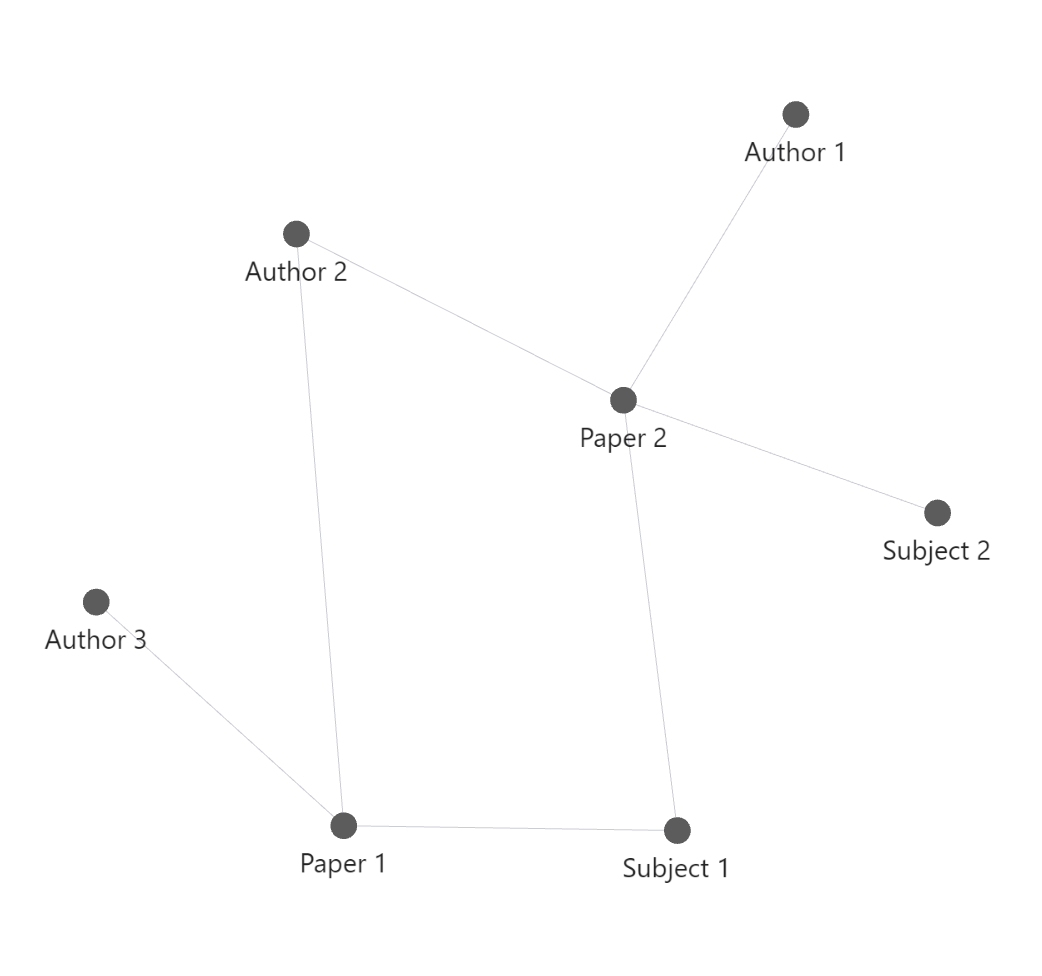
\includegraphics[width=10cm]{knowledgegraph.png}
    \caption{Example knowledge graph with dummy nodes}
\end{figure}

\subsubsection{Text-Content Graph}
For each paper, a Text-Content Graph will be constructed from its full text
(title, abstract, and body) to capture intra-paper semantic relationships. Key
entities and concepts (e.g., "vision transformer," "healthcare," "deep learning")
will be extracted as nodes using SciBERT-based Named Entity Recognition (NER)
\parencite{beltagy2019scibertpretrainedlanguagemodel} and KeyBERT \parencite{10295108}
for keyphrase identification. Edges will be defined based on relationships
identified through multiple methods: co-occurrence (entities appearing in the
same sentence or paragraph, weighted by frequency), dependency parsing
(syntactic relationships like "vision transformer improves healthcare,"
labeled accordingly), and semantic similarity (cosine similarity between
SciBERT embeddings of entities exceeding a threshold, e.g., 0.8). These
graphs will be built using NetworkX for in-memory processing, with each node
representing an entity/concept and each edge reflecting a contextual or syntactic
link within the paper.
\begin{figure}[H]
    \centering
    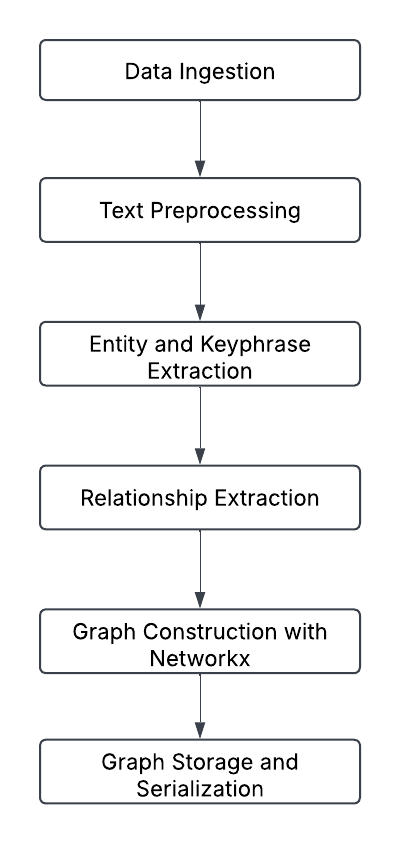
\includegraphics[width=5cm]{textcontentgraphflowchart.png}
    \caption{Text-Content Graph Flowchart}
\end{figure}

\subsubsection{Semantic Embeddings}
Semantic representations will be generated for the entire text of each paper
(title, abstract, and body) to fully capture its content and context. SciBERT,
a transformer model fine-tuned on scientific texts, will process the full text
in segments (e.g., 512-token chunks) due to its input constraints, producing
contextual embeddings (768-dimensional vectors) for each segment. These will be
averaged across segments to create a single content-based embedding per paper,
reflecting its scientific meaning. Simultaneously, TransR will embed each paper
based on its position in the knowledge graph, generating structural embeddings
(e.g., 100-dimensional vectors) that encode relationships like citations and
co-authorships. For each paper, the SciBERT
\parencite{beltagy2019scibertpretrainedlanguagemodel} and TransR
\parencite{10.3233/JIFS-202177} embeddings will be combined (e.g., concatenated or
weighted) into a unified vector representation. These vectors will be stored in a
vector database for efficient similarity search. The full corpus approach ensures
richer representations, capturing details from methods, results and discussions.
The database will be updated incrementally as new papers are added, recomputing
embeddings only for new documents to maintain scalability.
\begin{figure}[H]
    \centering
    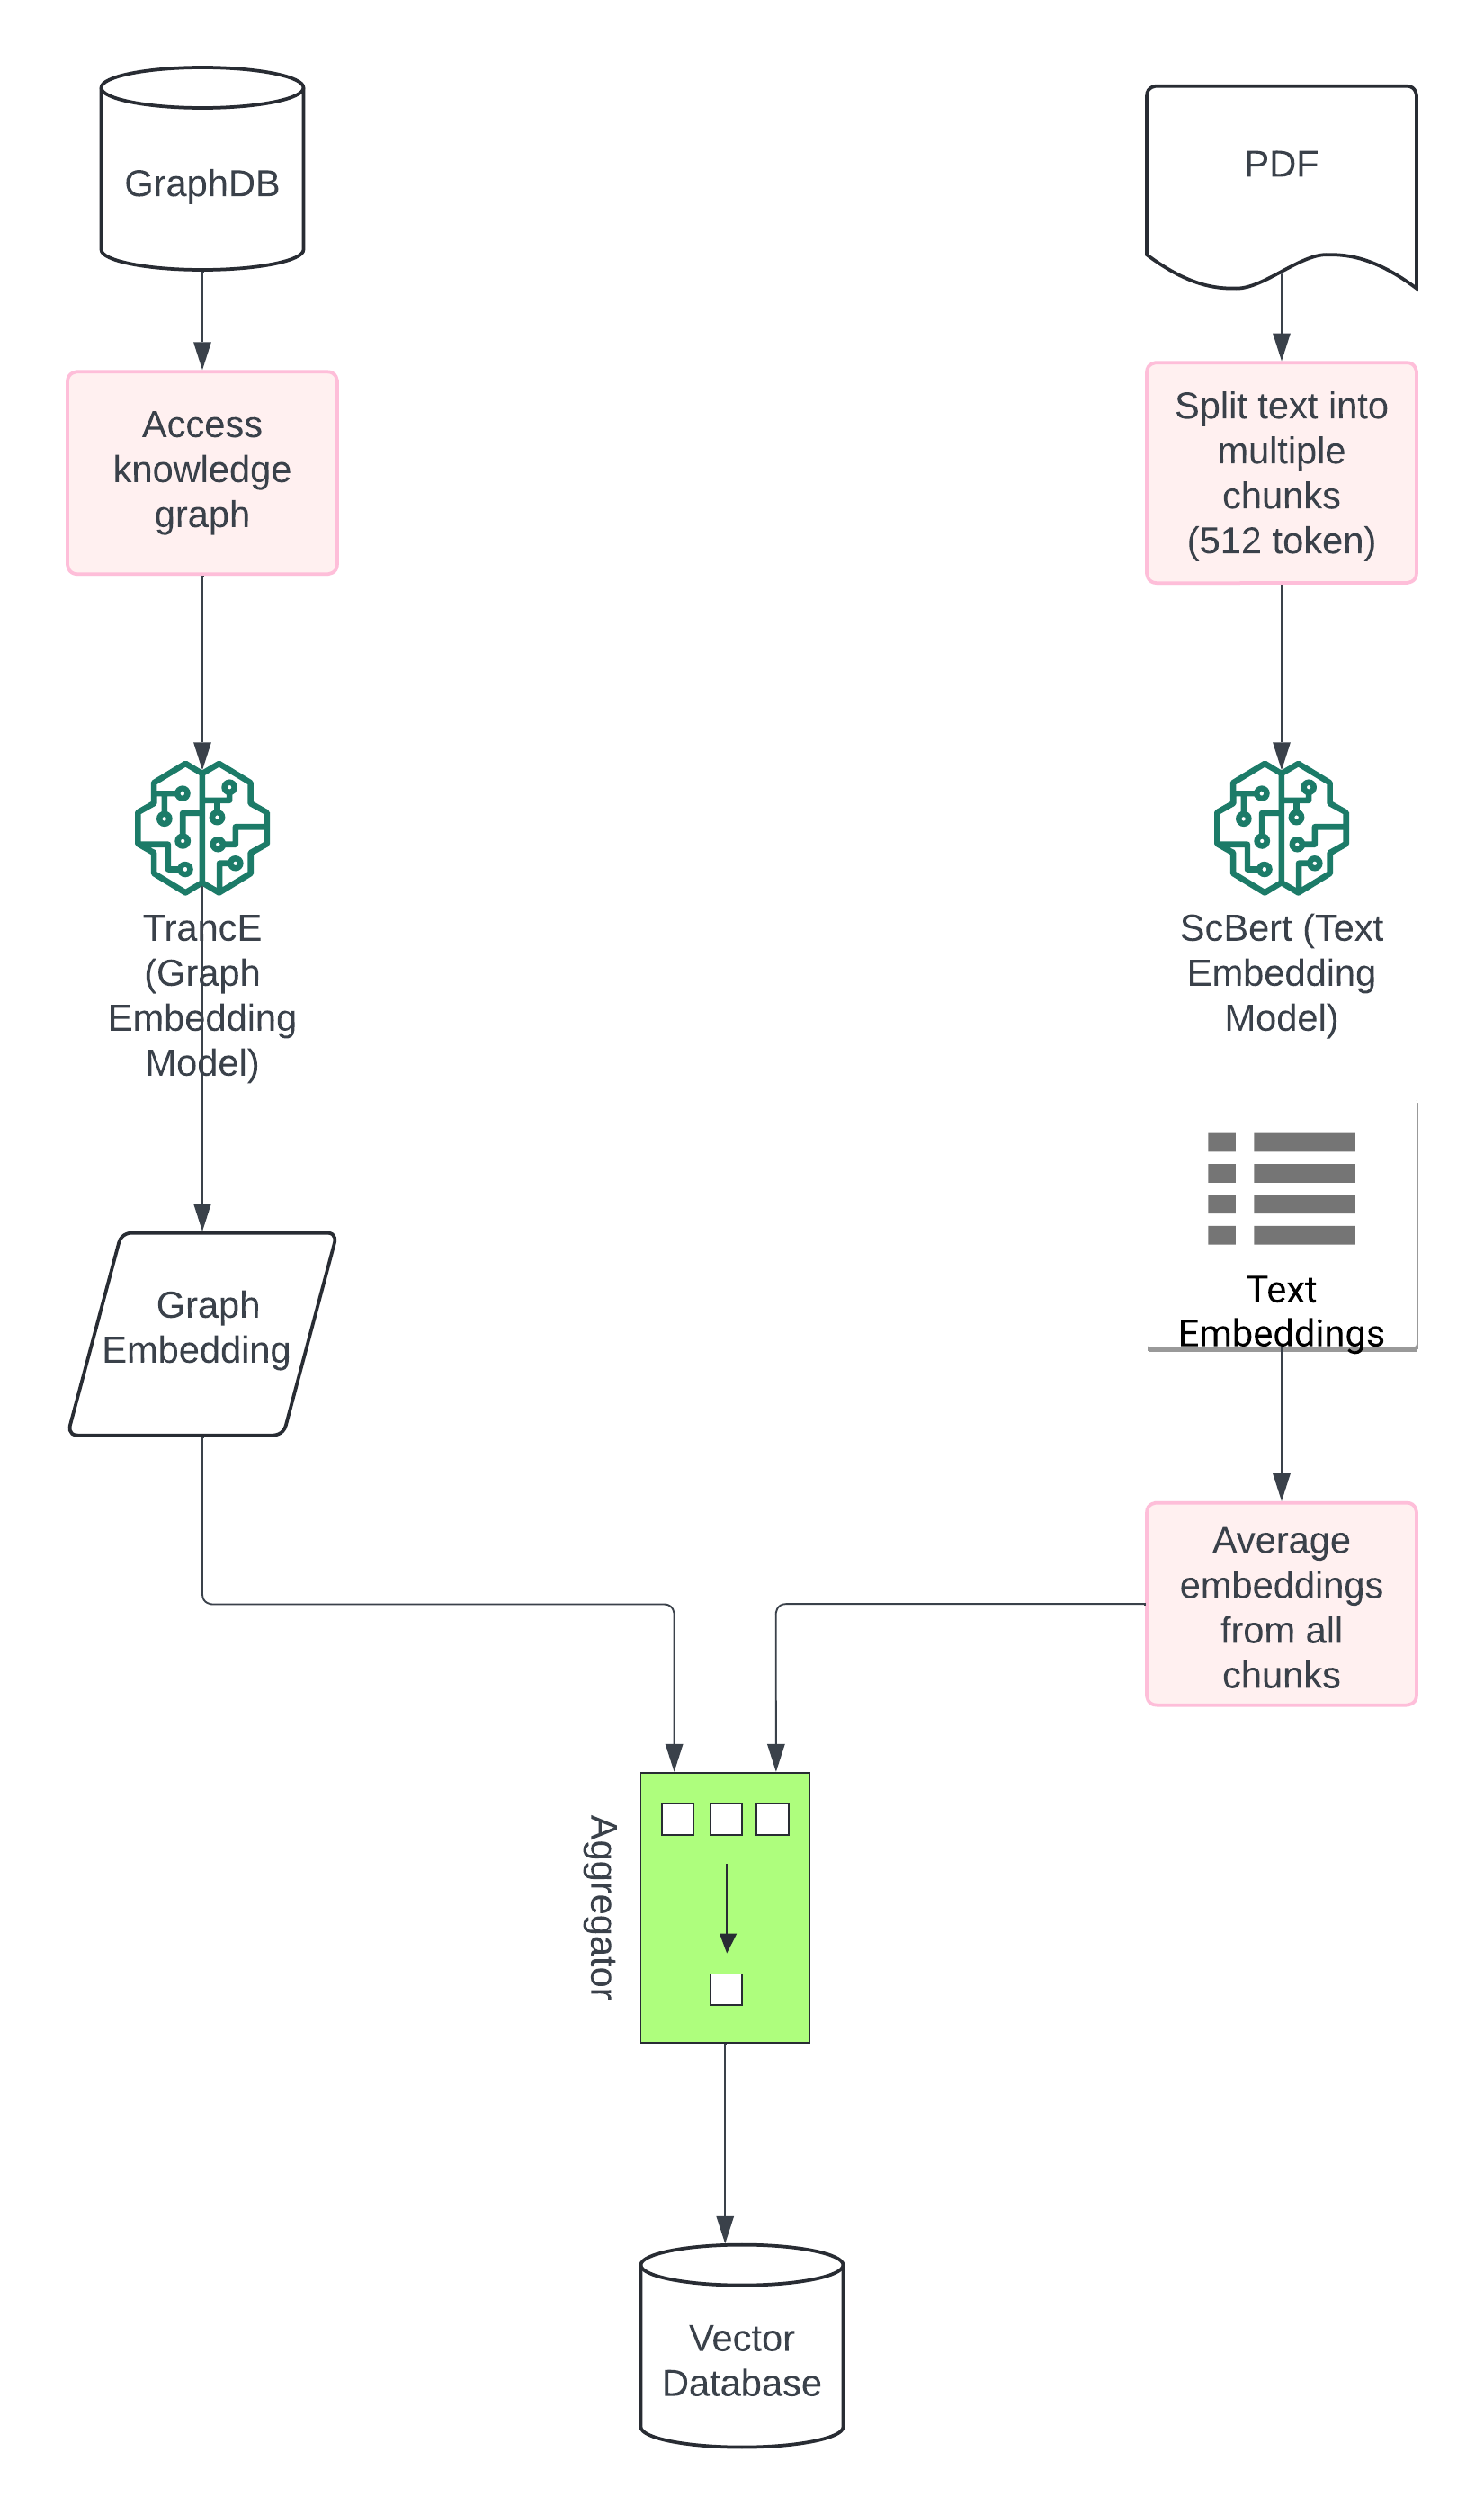
\includegraphics[width=7cm]{semanticembedding.png}
    \caption{Embedding generation pipeline}
\end{figure}
\newpage

\subsection{Generating Recommendation}
\begin{figure}[H]
    \centering
    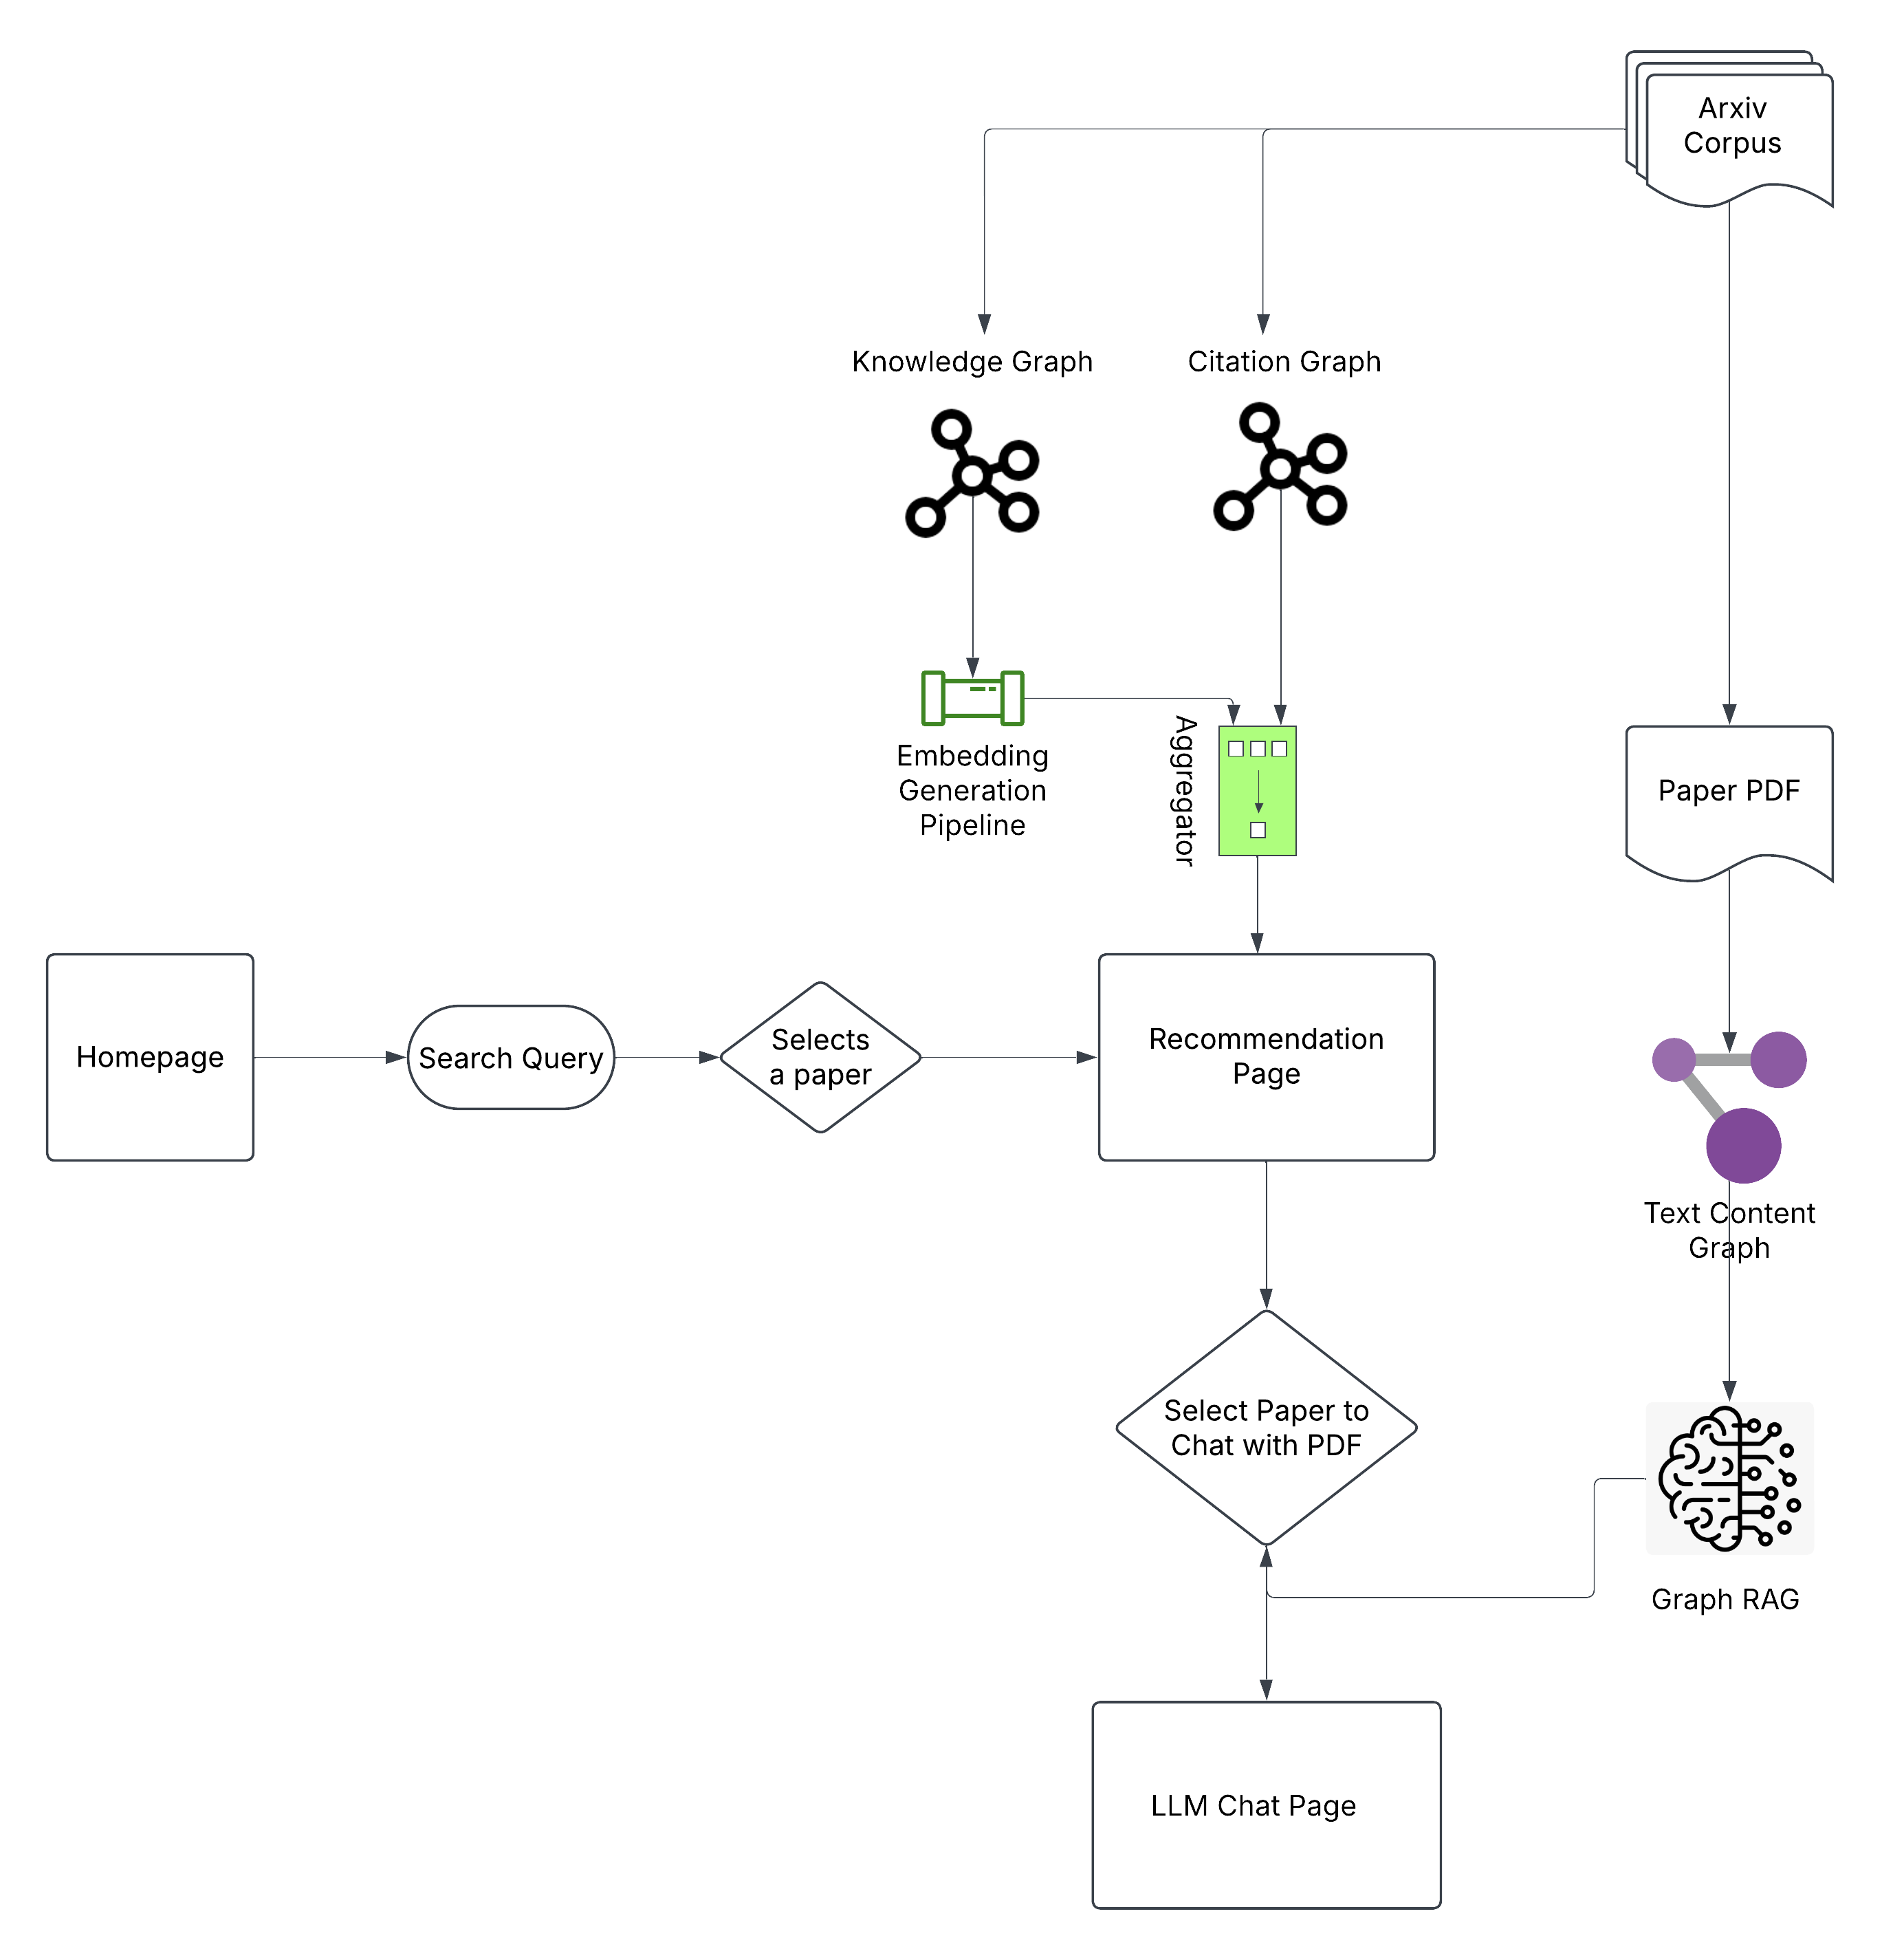
\includegraphics[width=15cm]{architecture.png}
    \caption{High-level System Architecture Overview}
\end{figure}

\subsubsection{Citation-Based Search}
This approach of generating recommendation is a path based approach where we will
simulate random walks on the citation graph and the papers with the most visits will
be recommended to the user. This approach ensures we suggest he most relevant paper.

\subsubsection{Semantic Search}
Semantic Search queries the vector database using a user input, embedding it with
SciBERT, and retrieving the top K papers based on cosine similarity of content
embeddings, supplemented by TransR embeddings for rational alignment. Using these
embedding will compute similarity measures and recommend the most relevant papers.

\subsubsection{Ranking}
Each candidate is scored using a weighted combination including Citation strength,
SciBERT similarity and TransR similarity. The top K papers are selected according
to need.

\subsection{GraphRAG Integration}
GraphRAG leverages the Text-Content Graph to enable the LLM to chat with the content
of a single PDF paper, providing an interactive question-answering feature.The
text-content graph constructed from the paper’s full text captures intra-paper
semantic relationships. The graph comprises nodes as key entities and concepts
and edges as relationships. Alongside this, the paper’s SciBERT embeddings, which
encode the full-text content into 768-dimensional vectors, are included to provide
detailed semantic context. The LLM processes this hybrid input within the Graph RAG
framework, reasoning over the text-content graph’s structure and the embeddings’
semantic depth. When a user poses a question, the LLM traverses the graph to identify
relevant relationships and uses the embeddings to extract precise content, generating
a natural language response. This integration empowers users to explore a paper’s
content interactively, offering a conversational interface.
\newpage

\section{System Requirement Specification}
\newpage

\section{Project Planning and Scheduling}
We are looking forward to completing the project in the time frame of 16 weeks by
distributing the tasks to each member of the group . We are planning to work on our own
on the weekdays and gather on the project day to discuss and compile the codes
collectively. The following Gantt chart shows the time allocation for different aspects of
our project
\newpage

\section{Expected Outcome}
The expected outcome of this project is a web application designed to revolutionize
academic literature discovery. The system will employ a hybrid approach that combines
citation networks and knowledge graphs to retrieve papers relevant to user queries.
Recommendations will be ranked based on citation impact and semantic similarity,
ensuring both influential and contextually relevant papers are prioritized.
Additionally, the integration of GraphRAG will enable users to interactively
explore and understand the content of papers, enhancing their research experience.
By addressing the limitations of current academic search platforms, this project aims
to significantly improve the efficiency and effectiveness of literature discovery
for researchers and students alike.
\newpage

\addcontentsline{toc}{section}{\textit{References}}
\printbibliography
\newpage

\end{document}
